\apendice{Especificación de Requisitos}
Este apéndice se subdivide en los diferentes requisitos necesarios para nuestro proyecto, en su realización y subdivisión. 
\section{Objetivos Generales}
\begin{enumerate}
\item Construcción de un cuestionario anónimo para la recogida de datos iniciales para ser utilizados en el entrenamiento de los sistemas de recomendación. 
\item Desarrollo de diferentes sistemas de recomendación, su entrenamiento en base a los datos recogidos y la devolución de las ponderaciones de las asignaturas no cursadas por un usuario. 
\item Desarrollo de una interfaz gráfica modo usuario para una mejor utilización de los mismos, de forma que las recomendaciones mostradas por el sistema de recomendación sean específicas para determinado usuario. 
\item Desarrollo de una interfaz gráfica modo administrador para la modificación, agregación o eliminación de diferentes calificaciones. 
\end{enumerate}
\section{Catálogo de Requisitos}
\begin{itemize}
\item RF-1. Recogida de datos\\ 
\begin{itemize}
\item RF-1.1. Creación de cuestionario anónimo.\\ 
\item RF-1.2. Distribución del cuestionario. \\ 
\item RF-1.3. Recogida de datos y su almacenamiento. 
\end{itemize}

\item RF-2. Desarrollo de los sistemas de recomendación\\ 
\begin{itemize}
\item RF-2.1. Recogida de datos de Drive. 
\item RF-2.2. Tratamiento de los datos. 
\item RF-2.3. Desarrollo del sistema de recomendación. 
\item RF-2.4. Devolución de las calificaciones. \item Guardado de los datos. 
\end{itemize}

\item RF-3. Desarrollo de una interfaz gráfica \\ 
\begin{itemize}
\item RF-3.1. Construcción de pestaña de inicio sesión.  
\item RF-3.2.Lectura de datos almacenados. \item Obtención de datos del registro de usuario. 
\item RF-3.3.Generación de recomendación de calificaciones. 
\item RF-3.4.Muestra de gráficos de calificaciones en diferentes asignaturas. 
\item RF-3.5.Muestra de gráficos auxiliares para mayor información al usuario. 
\item RF-3.6.Acceso a los datos generales en modo administrador. 
\end{itemize}
\end{itemize}

\section{Especificación de Requisitos}
\begin{itemize}


\item Construcción de ventana de inicio de sesión. 
\begin{itemize}
\item Construcción de botón de inicio sesión. 
\item Construcción de áreas para rellenar usuario y contraseña.  
\item Construcción de la funcionalidad para acceder a la Base de Datos. 
\item Construcción de la funcionalidad para validar usuario y contraseña. 
\end{itemize}

\item Construcción de la funcionalidad de la recogida,  guardado y  el tratamiento de los datos. 
\begin{itemize}
\item Construcción de la funcionalidad de recogida de datos de Drive. 
\item Construcción de la funcionalidad del tratamiento de los datos recogidos. 
\item Construcción de la funcionalidad para el guardado de los datos. 

\end{itemize}

\item Construcción de la pestaña inicial para rellenar el cuestionario para ponderar las asignaturas cursadas. 
\begin{itemize}
\item Construcción de la funcionalidad de los botones para seleccionar los cursos para ponderar sus asignaturas. 
\item Construcción de la funcionalidad para guardar en local los resultados introducidos. 
\item Construcción de la funcionalidad para poder modificar las ponderaciones introducidas. 
\end{itemize}

\item Construcción de las pestañas para la recomendación de las asignaturas. 
\begin{itemize}
\item Construcción de los botones  de selección del Sistema de Recomendación.
\item Construcción de funcionalidad para llamar al sistema de recomendación  seleccionado. 
\item Construcción de la funcionalidad para ejecutar el sistema de recomendación con los datos rellenados. 
\item Construcción de la funcionalidad para mostrar las calificaciones resultantes no cursadas. 
\item Construcción de la funcionalidad para mostrar gráficos de dicha recomendación. 
\end{itemize}

\item Construcción de la pestaña para la muestra de gráficos auxiliares. 
\begin{itemize}
\item Construcción de la funcionalidad para mostrar la media aritmética del curso. 
\item Construcción de la funcionalidad para mostrar gráficos auxiliares de las preferencias de las asignaturas. 
\end{itemize}

\end{itemize}

\section{Diagramas de Casos de Uso}
\subsection{Diagrama General}
El siguiente diagrama corresponde al  caso de uso general, junto con el diagrama extendido. ~\ref{fig:Diagrama_Caso_Uso_General}
\begin{figure}[h]
\centering
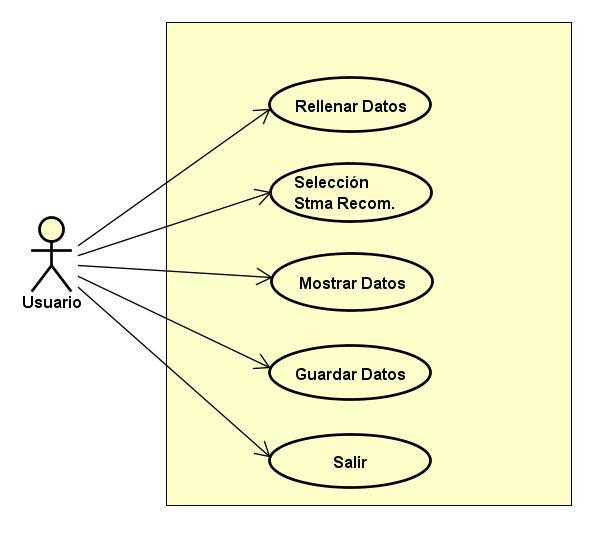
\includegraphics[width=0.90\textwidth]{Diagrama_Caso_Uso_General}
\caption{Diagrama de caso de uso General}
\label{fig:Diagrama_Caso_Uso_General}
\end{figure}

\section{Tablas de Casos de Uso Generales}
\subsection{Primer Caso de Uso}
La primera tabla corresponde al desarrollo del cuestionario anónimo y la recogida de datos para poder trabajar posteriormente con ellos. La siguiente tabla hace referencia al dicho caso de uso. \ref{tab:1}
\begin{table}[]
\caption{Tabla Caso de Uso 1}
\label{tab:1}
\resizebox{\textwidth}{!}{
\begin{tabular}{ lrrr }
\toprule
\textbf{Nombre} &   Recogida de Datos         \\ 
\textbf{Versión} & 1.0  \\ 
\textbf{Requisitos Funcionales}  & \begin{tabular}[c]{@{}l@{}}RF-1\\ RF-1.1\\ RF-1.2\\ RF-1.3\\\end{tabular}                                                                                                                  \\ 
\textbf{Descripción de Requisitos} & \begin{tabular}[r]{@{}l@{}}Se obtendrán los datos de forma anónima  para el entrenamiento\\ de los sistemas de recomendación\\\end{tabular}                                                                                                                    \\
\textbf{Precondiciones}     & No tiene \\
\textbf{Postcondiciones}         &  Se almacenarán los datos en una API de Google \\
\textbf{Autor}         & Clara Palacios Rodrigo \\
\textbf{Importancia}        &  Importante \\ \bottomrule
\end{tabular}
}
\end{table}

\subsection{Segundo Caso de Uso}
La segunda tabla corresponde con el desarrollo de los sistemas de recomendación. Para ello, se debe obtener los datos de la API de Drive, tratarlos y desarrollar los diferentes sistemas de recomendación. La siguiente tabla hace referencia a dicho caso de uso. ~\ref{tab:2}
\begin{table}[]
\caption{Tabla Caso de Uso 2}
\label{tab:2}
\resizebox{\textwidth}{!}{
\begin{tabular}{ lrrr }
\toprule
\textbf{Nombre} &   Desarrollo de los sistemas de recomendación        \\ 
\textbf{Versión} & 1.0  \\ 
\textbf{Requisitos Funcionales}  & \begin{tabular}[c]{@{}l@{}}RF-2\\ RF-2.1\\ RF-2.2\\ RF-2.3\\RF-2.4\end{tabular}                                                                                                                  \\ 
\textbf{Descripción de Requisitos} & \begin{tabular}[c]{@{}l@{}}Se permitirá el acceso a los datos globales para el sistema de recomendación\\  así como la obtención de los mismos.\\\end{tabular}                                                                                                                     \\
\textbf{Precondiciones}     & \begin{tabular}[c]{@{}l@{}} Disponer de los datos en Drive\\ Disponer de los Sistemas de Recomendación\\\end{tabular}                                                                                                                   \\
\textbf{Postcondiciones}         &  Devolución de los resultados \\
\textbf{Autor}         & Clara Palacios Rodrigo \\
\textbf{Importancia}        & Muy Importante \\ \bottomrule
\end{tabular}
}
\end{table}


\subsection{Tercer Caso de Uso}
La tercera tabla corresponde con  el desarrollo de la interfaz gráfica, así como la funcionalidad de los botones de la misma. De esta forma, se mostrarán los datos en la interfaz de acuerdo con el entrenamiento de los sistemas de recomendación con los datos introducidos por el usuario, así como gráficos correspondientes a dichos datos y a los resultados obtenidos por el sistema de recomendación seleccionado. La siguiente tabla hace referencia a dicho caso de uso. ~\ref{tab:3}
\begin{table}[]
\caption{Tabla Caso de Uso 3}
\label{tab:3 }
\resizebox{\textwidth}{!}{
\begin{tabular}{ lrrr }
\toprule
\textbf{Nombre} &  Desarrollo de una interfaz gráfica  \\ 
\textbf{Versión} & 1.0  \\ 
\textbf{Requisitos Funcionales}  & \begin{tabular}[c]{@{}l@{}}RF-3\\ RF-3.1\\ RF-3.2\\ RF-3.3\\RF-3.4\\RF-3.5\\RF-3.6\end{tabular}                                                                                                                  \\ 
\textbf{Descripción de Requisitos} & \begin{tabular}[c]{@{}l@{}}Se recogerán los datos al usuario y se mostrarán gráficos y resultados\\obtenidos del sistema de recomendación escogido.\\\end{tabular}                                                                                                                     \\
\textbf{Precondiciones}     & \begin{tabular}[c]{@{}l@{}}Disponer de una interfaz gráfica.\\Haber solicitado los datos al usuario.\end{tabular}                                                                                                                     \\
\textbf{Postcondiciones}         &  Ninguna \\
\textbf{Autor}         & Clara Palacios Rodrigo \\
\textbf{Importancia}        & Muy Importante \\ \bottomrule
\end{tabular}
}
\end{table}


\section{Requisitos Funcionales}
Esta sección consistirá en el desarrollo de los requisitos funcionales de forma detallada explicando 
